\documentclass[aspectratio=169]{beamer}
\usetheme{Madrid}
\usecolortheme{beaver}
\usepackage[utf8]{inputenc}
\usepackage[T1]{fontenc}
\usepackage{tikz}
\usepackage{amssymb}
\usepackage{graphicx}
\setbeamertemplate{navigation symbols}{}
\setbeamercolor{title}{fg=white,bg=cyan!60!black}
\setbeamercolor{frametitle}{fg=white,bg=cyan!50!black}
\setbeamercolor{block title}{bg=cyan!15,fg=black}
\setbeamercolor{block body}{bg=cyan!5,fg=black}

\title{Story Studio 4 — Remember Things}
\subtitle{Variables — a story that remembers the reader's choice}
\author{ByteForge --- Grade 7 --- Game Maker --- Week Overview}
\date{}

\begin{document}

\begin{frame}
    \titlepage
\end{frame}

\begin{frame}{This Week's Plan}
    \begin{itemize}
        \item Lesson 1: Remember the Choice
        \item Lesson 2: Two Details, One Story
        \item Lesson 3: The Choice Updates
        \item[$\bigstar$] BOSS --- The Choice Remembered (\texttt{lessonBoss.tex})
    \end{itemize}
\end{frame}

\begin{frame}{Real-World Example}
    \Large
    Your shopping cart total, a video's "watched 12:34 of 20:00" progress, a game's remembered high score between sessions — every one of these is a variable persisting a value. Minecraft's hunger bar (20 drumsticks, dropping as you act, refilling as you eat) is a variable your character carries constantly.
\end{frame}


\begin{frame}{Image}
    \begin{center}
    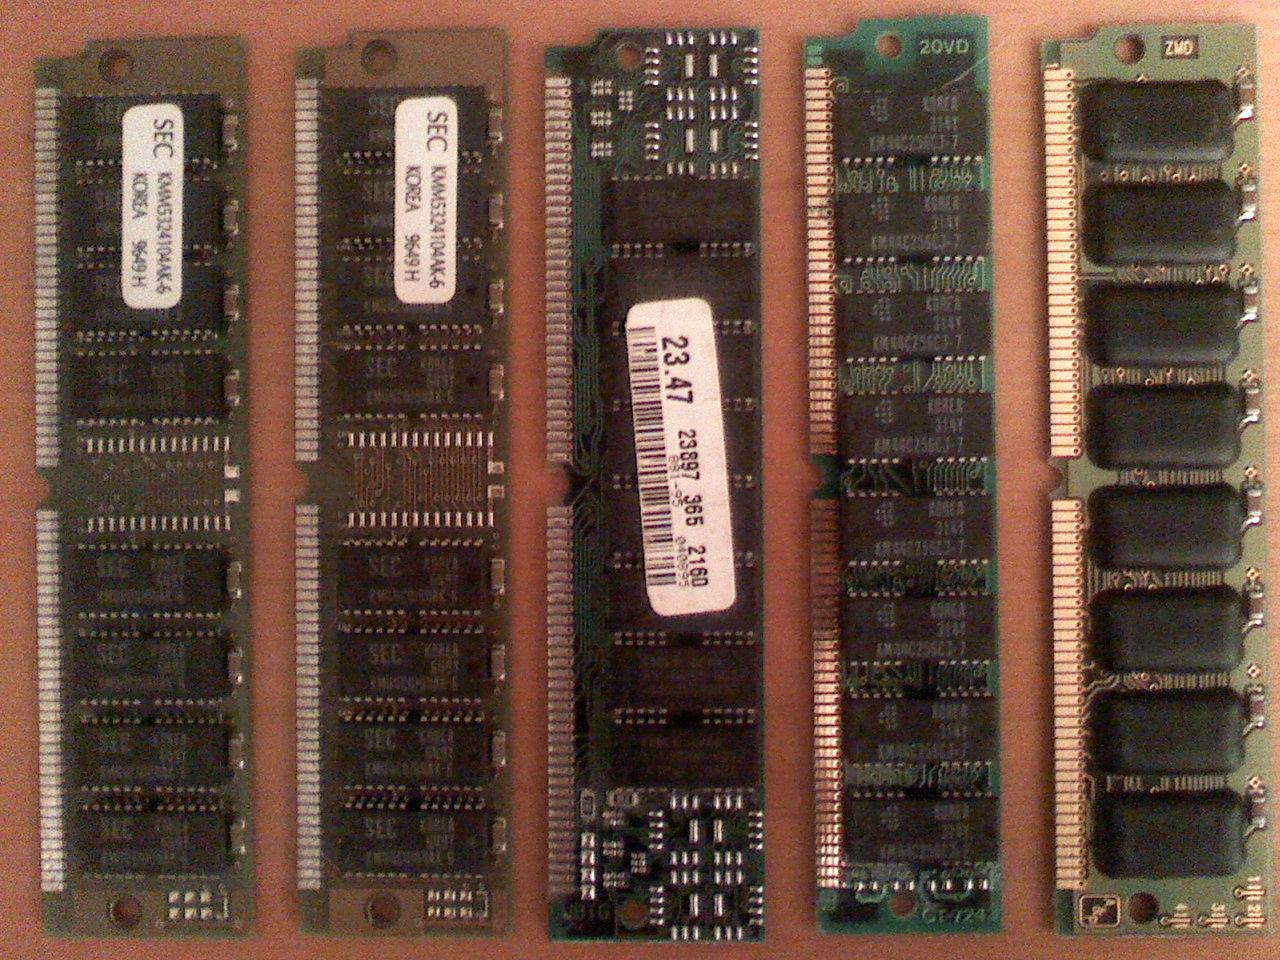
\includegraphics[width=0.55\textwidth]{../images/ram.jpg}

    \small RAM modules, public domain (PD-self), via Wikimedia Commons
    \end{center}
\end{frame}

\begin{frame}{Let Them Discover}
    \Large
    Name three things a website "remembers" about you between visits (logged-in name, cart items, dark mode setting). For each, is it stored as a variable in that one page-visit, or does it need to persist even after you close the tab?
\end{frame}

\begin{frame}{Files in This Folder}
    \small
    \begin{itemize}
        \item \texttt{lesson1.tex} --- Remember the Choice
        \item \texttt{lesson2.tex} --- Two Details, One Story
        \item \texttt{lesson3.tex} --- The Choice Updates
        \item \texttt{lessonBoss.tex} --- BOSS: The Choice Remembered
    \end{itemize}
    \vspace{0.5em}
    \normalsize Each lesson file is its own short deck --- open the one for
    the specific day you're teaching, not this whole overview.
\end{frame}

\end{document}
